\documentclass[portrait,draft,a0paper]{baposter}
%\documentclass[a4shrink,portrait,final]{baposter}
% Usa a4shrink for an a4 sized paper.

\tracingstats=2

% special 
\usepackage{ifthen}
\usepackage{ifpdf}
\usepackage{float}
\usepackage{color}

% fonts
\usepackage{latexsym}
\usepackage{amsmath} 
\usepackage{amssymb} 
\usepackage{bm}
\usepackage{wasysym}


\ifpdf
\usepackage{graphicx}
\usepackage{epstopdf}
\else
\usepackage{graphicx}
\usepackage{epsfig}
\fi


\graphicspath{{figures/},{PROG/figures/}}


%%%%%%%%%%%%%%%%%%%%%%%%%%%%%%%%%%%%%%%%%%%%%%%%%%%%%%%%%%%%%%%%


% NEW 
\newcommand{\abs}[1]{\left|#1\right|}
\newcommand{\Prob}{\mbox{Prob}\,}
\newcommand{\erf}{\mbox{erf}\,}
\newcommand{\barline}[1]{#1}

% math symbols I
\newcommand{\sinc}{\mbox{sinc}}
\newcommand{\const}{\mbox{const}}
\newcommand{\trc}{\mbox{trace}}
\newcommand{\intt}{\int\!\!\!\!\int }
\newcommand{\ointt}{\int\!\!\!\!\int\!\!\!\!\!\circ\ }
\newcommand{\ar}{\mathsf r}
\newcommand{\im}{\mbox{Im}}
\newcommand{\re}{\mbox{Re}}

% math symbols II
\newcommand{\eexp}{\mbox{e}^}
\newcommand{\bra}{\left\langle}
\newcommand{\ket}{\right\rangle}

% Mass symbol
\newcommand{\mass}{\mathsf{m}} 
\newcommand{\Mass}{\mathsf{M}} 

% more math commands
\newcommand{\tbox}[1]{\mbox{\tiny #1}}
\newcommand{\bmsf}[1]{\bm{\mathsf{#1}}} 
%\newcommand{\amatrix}[1]{\matrix{#1}} 
\newcommand{\amatrix}[1]{\begin{matrix} #1 \end{matrix}} 
\newcommand{\pd}[2]{\frac{\partial #1}{\partial #2}}

% equations
\newcommand{\mylabel}[1]{\label{#1}} 
%\newcommand{\mylabel}[1]{\textcolor{blue}{[#1]}\label{#1}} 
\newcommand{\beq}{\begin{eqnarray}}
\newcommand{\eeq}{\end{eqnarray}} 
\newcommand{\be}[1]{\begin{eqnarray}\ifthenelse{#1=-1}{\nonumber}{\ifthenelse{#1=0}{}{\mylabel{e#1}}}}
\newcommand{\ee}{\end{eqnarray}} 

% arrangement
\newcommand{\drawline}{\begin{picture}(500,1)\line(1,0){500}\end{picture}}
\newcommand{\bitem}{$\bullet$ \ \ \ }
\newcommand{\Cn}[1]{\begin{center} #1 \end{center}}
\newcommand{\mpg}[2][1.0\hsize]{\begin{minipage}[b]{#1}{#2}\end{minipage}}
\newcommand{\mpgt}[2][1.0\hsize]{\begin{minipage}[t]{#1}{#2}\end{minipage}}
\newcommand{\putgraph}[2][width=0.30\hsize]{\includegraphics[#1]{#2}}

% more
%\newcommand{\Eq}[1]{Eq.\!\!~(\ref{#1})}
%\newcommand{\Fig}[1]{Fig.\!\!~\ref{#1}}  
\newcommand{\Eq}[1]{\textcolor{blue}{Eq.\!\!~(\ref{#1})}} 
\newcommand{\Fig}[1]{\textcolor{blue}{Fig.}\!\!~\ref{#1}} 
\newcommand{\hide}[1]{} %{\textcolor{red}{[hidden text]}} %{}
\newcommand{\rmrk}[1]{\textcolor{red}{#1}}


%%%%%%%%%%%%%%%%%%%%%%%%%%%%%%%%%%%%%%%%%%%%%%%%%%%%%%%%%%%%%%%%%%%%%%%%%%%

% extra math commands by jarondl
\newcommand{\inner}[2]{\left \langle #1 \middle| #2\right\rangle} % Inner product
\newcommand{\avgangle}[1]{\left\langle #1 \right\rangle} % Average <x>

%fminipage using fancybox package
\newenvironment{fminipage}%
  {\begin{Sbox}\begin{minipage}}%
  {\end{minipage}\end{Sbox}\fbox{\TheSbox}}


    

%%%%%%%%%%%%%%%%%%%%%%%%%%%%%%%%%%%%%%%%%%%%%%%%%%%%%%%%%%%%%%%%%%%%%%%%%%%%%%
%%% Begin of Document
%%%%%%%%%%%%%%%%%%%%%%%%%%%%%%%%%%%%%%%%%%%%%%%%%%%%%%%%%%%%%%%%%%%%%%%%%%%%%%

\begin{document}

%%%%%%%%%%%%%%%%%%%%%%%%%%%%%%%%%%%%%%%%%%%%%%%%%%%%%%%%%%%%%%%%%%%%%%%%%%%%%%
%%% Here starts the poster
%%%---------------------------------------------------------------------------
%%% Format it to your taste with the options
%%%%%%%%%%%%%%%%%%%%%%%%%%%%%%%%%%%%%%%%%%%%%%%%%%%%%%%%%%%%%%%%%%%%%%%%%%%%%%
% Define some colors
\definecolor{silver}{cmyk}{0,0,0,0.3}
\definecolor{yellow}{cmyk}{0,0,0.9,0.0}
\definecolor{reddishyellow}{cmyk}{0,0.22,1.0,0.0}
\definecolor{black}{cmyk}{0,0,0.0,1.0}
\definecolor{darkYellow}{cmyk}{0,0,1.0,0.5}
\definecolor{darkSilver}{cmyk}{0,0,0,0.1}

\definecolor{lightyellow}{cmyk}{0,0,0.3,0.0}
\definecolor{lighteryellow}{cmyk}{0,0,0.1,0.0}
\definecolor{lighteryellow}{cmyk}{0,0,0.1,0.0}
\definecolor{lightestyellow}{cmyk}{0,0,0.05,0.0}

%%
%\background{
%  \begin{tikzpicture}[remember picture,overlay]%
%    \draw (current page.north west)+(-2em,2em) node[anchor=north west] {\includegraphics[height=1.1\textheight]{silhouettes_background}};
%  \end{tikzpicture}%
%}
\typeout{Poster Starts}



\begin{poster}%
  % Poster Options
  {
  bgColorOne=lightgray!30,
  %bgColorTwo=yellow,
  headerheight=0.1\textheight,
  columns=3,
  headershade=plain,
  headerColorOne=green!40,
  boxColorOne=lightgray!75,
  headershape=smallrounded,
  textborder=roundedsmall,
  linewidth=0.5pt,
  borderColor=green,
  headerborder=open,
  eyecatcher=false,
  background=plain
}
  % Eye Catcher
  {\includegraphics[width=10em]{D1077}} % No eye catcher for this poster. (eyecatcher=no above). If an eye catcher is present, the title is centered between eye-catcher and logo.
  % Title
  {\sf 
Transport in "sparse" networks:\\ 
From linear response to effective range hopping.
  }
  % Authors
  {\sf
  \vspace{2em}  {Yaron de Leeuw, Doron Cohen\\Ben-Gurion University of the Negev}%\\ 
%                Physics Department \\
%                 Ben-Gurion University of the Negev, \\
%                Beer-Sheva, Israel\\
%                \texttt{jarondl@bgu.ac.il}}
  }
  % University logo
  {\hspace{1em}
\includegraphics[height=10em]{BGU}\
  }

  \tikzstyle{light shaded}=[top color=baposterBGtwo!30!white,bottom color=baposterBGone!30!white,shading=axis,shading angle=30]


%%%%%%%%%%%%%%%%%%%%%%%%%%%%%%%%%%%%%%%%%%%%%%%%%%%%%%%%%%%%%%%%%%%%%%%%%%%%%%
%%% Now define the boxes that make up the poster
%%%---------------------------------------------------------------------------
%%% Each box has a name and can be placed absolutely or relatively.
%%% The only inconvenience is that you can only specify a relative position 
%%% towards an already declared box. So if you have a box attached to the 
%%% bottom, one to the top and a third one which should be in between, you 
%%% have to specify the top and bottom boxes before you specify the middle 
%%% box.
%%%%%%%%%%%%%%%%%%%%%%%%%%%%%%%%%%%%%%%%%%%%%%%%%%%%%%%%%%%%%%%%%%%%%%%%%%%%%%


%%%%%%%%%%%%%%%%%%%%%%%%%%%%%%%%%%%%%%%%%%%%%%%%%%%%%%%%%%%%%%%%%%%%%%%%%%%%%%
  \headerbox{The model}{name=model,column=0,row=0}{
%%%%%%%%%%%%%%%%%%%%%%%%%%%%%%%%%%%%%%%%%%%%%%%%%%%%%%%%%%%%%%%%%%%%%%%%%%%%%%
{}

We consider 1D, quasi-1D or 2D network with:
\begin{align*}
\frac{dp_n(t)}{dt} = \sum_m w_{nm} p_m(t)
\end{align*}
With $w_{nm}$ for the random site model:
\beq
w_{nm} =   \eexp{-|x_n-x_m|/\xi}  
\eeq
%
In the 1D case we consider also the following banded lattice model
%
\beq
w_{nm}  =   w_0  \eexp{-\epsilon_{nm}}  B(n-m)
\eeq


}
%%%%%%%%%%%%%%%%%%%%%%%%%%%%%%%%%%%%%%%%%%%%%%%%%%%%%%%%%%%%%%%%%%%%%%%%%%%%%%
  \headerbox{Diffusion}{name=diffusion,column=0, below=model}{
%%%%%%%%%%%%%%%%%%%%%%%%%%%%%%%%%%%%%%%%%%%%%%%%%%%%%%%%%%%%%%%%%%%%%%%%%%%%%%
{}

The long time dynamics are charectrized by the spreading $S(t)$, the survival probability $\mathcal{P}(t)$ and the spectral counting of states $\mathcal{N}(t)$. In the case of diffusion these are:
\begin{align}
S(t) &= \left\langle r^2(t) \right\rangle  =  (2d)Dt\ \\
\mathcal{P}(t) \quad &= \quad  \frac{1}{\left({4\pi D t}\right)^{d/2}} \\
\mathcal{N}(\lambda)  &\propto\left[\frac{\lambda}{D}\right]^{d/2} 
\end{align}

 }

%%%%%%%%%%%%%%%%%%%%%%%%%%%%%%%%%%%%%%%%%%%%%%%%%%%%%%%%%%%%%%%%%%%%%%%%%%%%%%
  \headerbox{The $1d$ chain model}{name=chain,column=0,below=diffusion}{
%%%%%%%%%%%%%%%%%%%%%%%%%%%%%%%%%%%%%%%%%%%%%%%%%%%%%%%%%%%%%%%%%%%%%%%%%%%%%%
{} In the $1d$ chain model, the location of each site has a uniform random distribution on a $1d$ line.

The rates are calculated according to $w_{nm} = w_0 \exp(-|r_m-r_n|/\xi)$, with only nearest neighbor transitions
($b=1$). We can convert the spacing distribution to rate distribution, and, making the analogy with adding connectors in series, we obtain:
\beq
D = D[w_n] = \left( \frac{1}{N} \sum_n \frac{1}{w_n} \right)^{-1} 
 =  \frac{s-1}{s} \, w_0
\eeq
for $s>1$, with $s=\xi/r_0$. For $0<s<1$, there is a sub diffusive regime, where the survival probability and spreading are:
\beq
S(t) \ \ &\propto& \ \ t^{2s/(1+s)}   \\ 
\mathcal{P}(t) \ \ &\propto& \ \ t^{-s/(1+s)}
\eeq
 These are exact analytic results, based on work by Shlomo Alexander, and they are summed up in panel (a) of figure \ref{fig:alexander}.
  \vspace{0.3em}
  }

%%%%%%%%%%%%%%%%%%%%%%%%%%%%%%%%%%%%%%%%%%%%%%%%%%%%%%%%%%%%%%%%%%%%%%%%%%%%%%
  \headerbox{Effective Range Hopping}{name=alexander,column=0,below=chain, above=bottom}{
%%%%%%%%%%%%%%%%%%%%%%%%%%%%%%%%%%%%%%%%%%%%%%%%%%%%%%%%%%%%%%%%%%%%%%%%%%%%%%
{}
The linear response theorem will not hold for very "sparse" systems, because only percolating 
connections contribute to the transport. We define a percolation limit by requiring :
\beq
\iint_{w(r,\epsilon)>w*} \rho(r,\epsilon)drd\epsilon  =  p_c
\eeq
with $p_c$ of order unity.

Then we calculate $D$ as follows:

\beq
D_{\tbox{ERH}}[\bm{w}]  = \frac{1}{4}\iint \min\{w(r,\epsilon),w^*\}  r^2   \rho(r,\epsilon) d\epsilon dr
\eeq
%
}
%%%%%%%%%%%%%%%%%%%%%%%%%%%%%%%%%%%%%%%%%%%%%%%%%%%%%%%%%%%%%%%%%%%%%%%%%%%%%%
  \headerbox{Diffusion as a function of sparsity}{name=alexander,column=1,span=2,row=0}{
%%%%%%%%%%%%%%%%%%%%%%%%%%%%%%%%%%%%%%%%%%%%%%%%%%%%%%%%%%%%%%%%%%%%%%%%%%%%%%
{}  

\begin{figure}[H]
  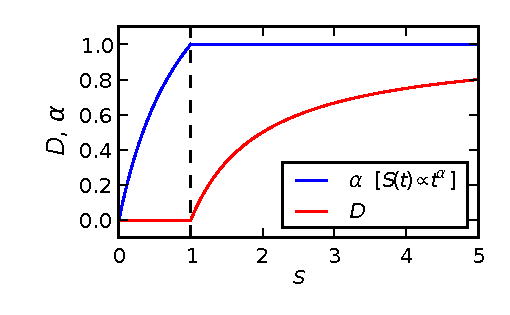
\includegraphics[width=0.45\textwidth]{alexander}
  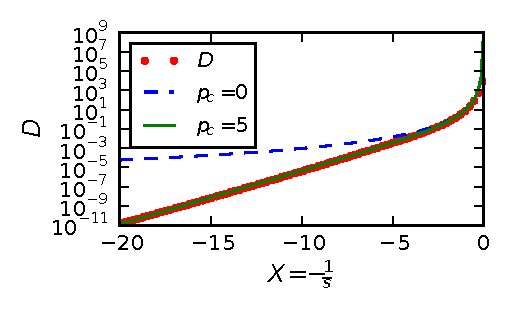
\includegraphics[width=0.45\textwidth]{ERH}
\caption{On the left: theoretical $1d$ chain model. On the right: the $2d$ results. In the $2d$ plot, on the right, we see the diffusion coefficient, numerical spectral analysis results vs ERH. The $Y$ axis is $D$ in logarithmic scale, while the $X$ axis is $X=-1/s$. }
\label{fig:alexander}
\end{figure}

  \vspace{0.3em}
  }


%%%%%%%%%%%%%%%%%%%%%%%%%%%%%%%%%%%%%%%%%%%%%%%%%%%%%%%%%%%%%%%%%%%%%%%%%%%%%%
  \headerbox{Banded Networks}{name=banded,column=1,span=2,above=bottom}{
%%%%%%%%%%%%%%%%%%%%%%%%%%%%%%%%%%%%%%%%%%%%%%%%%%%%%%%%%%%%%%%%%%%%%%%%%%%%%%
%If we had an ordered lattice, then the exact result for $D$ would be 
%
%\beq
%D  =  D_{\tbox{LRT}}[\bm{w}]   =  \frac{1}{2d}\iint w(r,\epsilon) \ r^2  \ \rho(r,\epsilon) \ d\epsilon dr 
%\eeq
%
%This expression is strictly {\em linear}.
%For the infinite temperature variation of 2D random site model we get  
%
%\beq
%D \ \ = \ \ 3\pi \, s^4 \, w_0
%\eeq
%
Now we consider quasi-1d networks, in which there is a band profile, meaning each site is connected to $b$ neighbor sites. The rates depend exponentialy on a random variable with a uniform distribution $[-\sigma,0]$.
\begin{figure}[H]
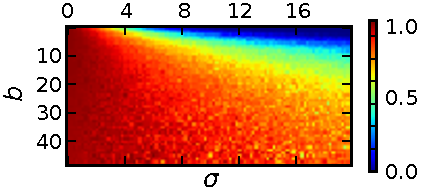
\includegraphics[height=10em]{resnet_new}
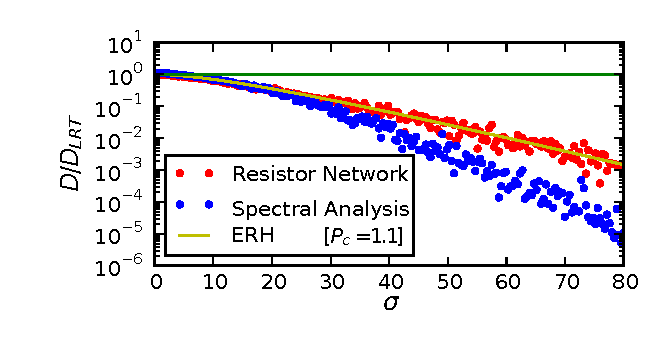
\includegraphics[height=10em]{banded_b10}
\caption{$D$ as calculated using the resistor network method. On the left, for many values of $b$ and $\sigma$, and on the right for $b=10$.}
\end{figure}

}
%%%%%%%%%%%%%%%%%%%%%%%%%%%%%%%%%%%%%%%%%%%%%%%%%%%%%%%%%%%%%%%%%%%%%%%%%%%%%%
 % \headerbox{ERH}{name=erh,column=2,below=alexander}{
%%%%%%%%%%%%%%%%%%%%%%%%%%%%%%%%%%%%%%%%%%%%%%%%%%%%%%%%%%%%%%%%%%%%%%%%%%%%%%
%The linear response theorem will not work for ${s<1}$ because sparse contribution 
%of strongly coupled sites do not contribute to the transport. 
%Only percolating trajectories do have a contribution. The Effective-Range-Method is
%an approximation that takes connectivity into account. We define the effective rate 
%through the requirement 
%
%\beq
%\iint_{w(r,\epsilon)>w*} \rho(r,\epsilon)drd\epsilon  =  p_c, 
%\ \mbox{with $p_c$ of order unity}
%\eeq
%
%Then we calculate $D$ as follows:
%
%\beq
%D \ \ = \ \ D_{\tbox{ERH}}[\bm{w}]  \ \ = \ \ \frac{1}{4}\iint \min\{w(r,\epsilon),w^*\} \ r^2  \ \rho(r,\epsilon) \ d%\epsilon dr
%\eeq
%
%This is similar to the LRT estimate, with network that has $w_{nm}$ 
%that are equal or smaller to the original values. The "suppressed" 
%connectors are those that are too sparse to form percolating trajectories. 
%Note that this expression, is {\em semi-linear} 
%rather than linear.
 
%}

%%%%%%%%%%%%%%%%%%%%%%%%%%%%%%%%%%%%%%%%%%%%%%%%%%%%%%%%%%%%%%%%%%%%%%%%%%%%%%
  \headerbox{Eigenvalue distributions}{name=eigvals,column=1,span=2,above=banded, below=alexander}{
%%%%%%%%%%%%%%%%%%%%%%%%%%%%%%%%%%%%%%%%%%%%%%%%%%%%%%%%%%%%%%%%%%%%%%%%%%%%%%
%%%%%%%%%%%%%%%%%%5
\begin{figure}[H]
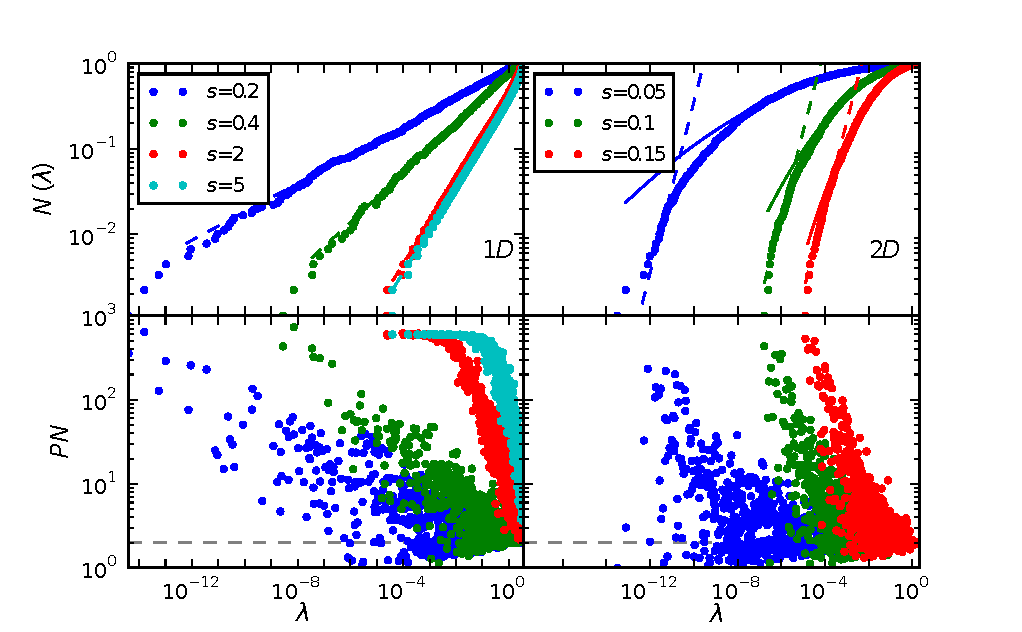
\includegraphics[clip, width=0.95\textwidth]{four_panels}
\caption{ Spectral properties for $1D$ and $2D$. The upper panels show the cummulative density of the eigenmodes, while the lower panels present the participation number of each mode. Modes with high participation numbers are extended and are more important for the long term behaviour. There is a striking difference between the $1d$ and $2d$ cases. For $1d$, the slope for sparse models ($s<1$) is less than $\frac{1}{2}$, meaning we have sub-diffusion. In the $2d$ case, the low-$\lambda$ slope is always $1$, which correspondes to normal diffusion.} \label{fig:exp_2d_D_vs_subD}
\end{figure}
}



\end{poster}

\end{document}
